\title{CS 361 - Concurrent Programming \\ Assignment 3}
\author{Dennis George}
\date{5/11/2021}
\documentclass[12pt]{article}
\usepackage[utf8]{inputenc}
\usepackage[english]{babel}
\usepackage{hyperref}
\usepackage{titling}
\usepackage{float}
\usepackage{mathtools}
\usepackage{enumitem}
\usepackage{amsmath}
\usepackage{upgreek}
\usepackage{tikz}
\usepackage{forest}
\usepackage{indentfirst}
\usepackage[margin=0.7in]{geometry}
\usepackage[document]{ragged2e}

\setlength{\parindent}{10ex}
\setlength{\parskip}{1em}

\renewcommand\maketitlehooka{\null\mbox{}\vfill}
\renewcommand\maketitlehookd{\vfill\null}


\begin{document}
\maketitle
    \section{Part 1 - Chapter3 Problem 5}

        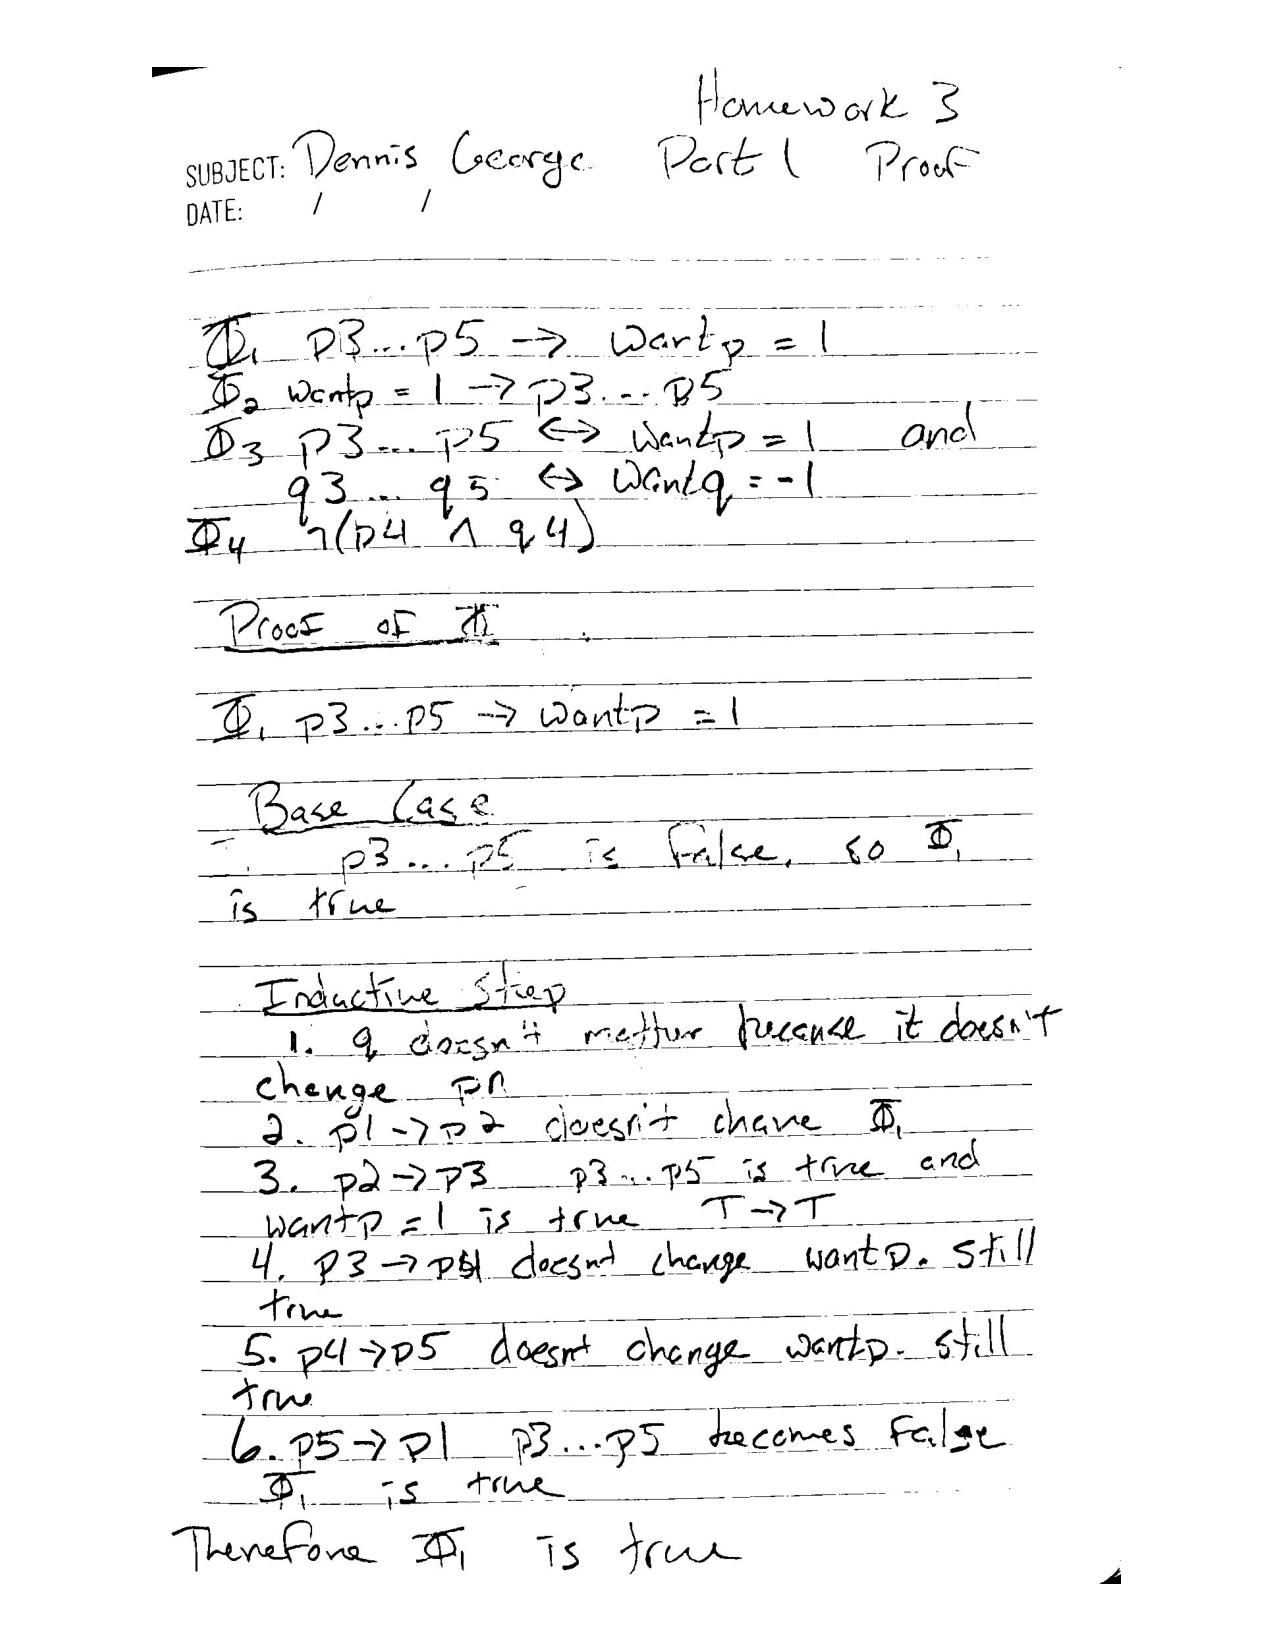
\includegraphics[scale=0.8]{Assignment3/1.pdf}
        \newpage
        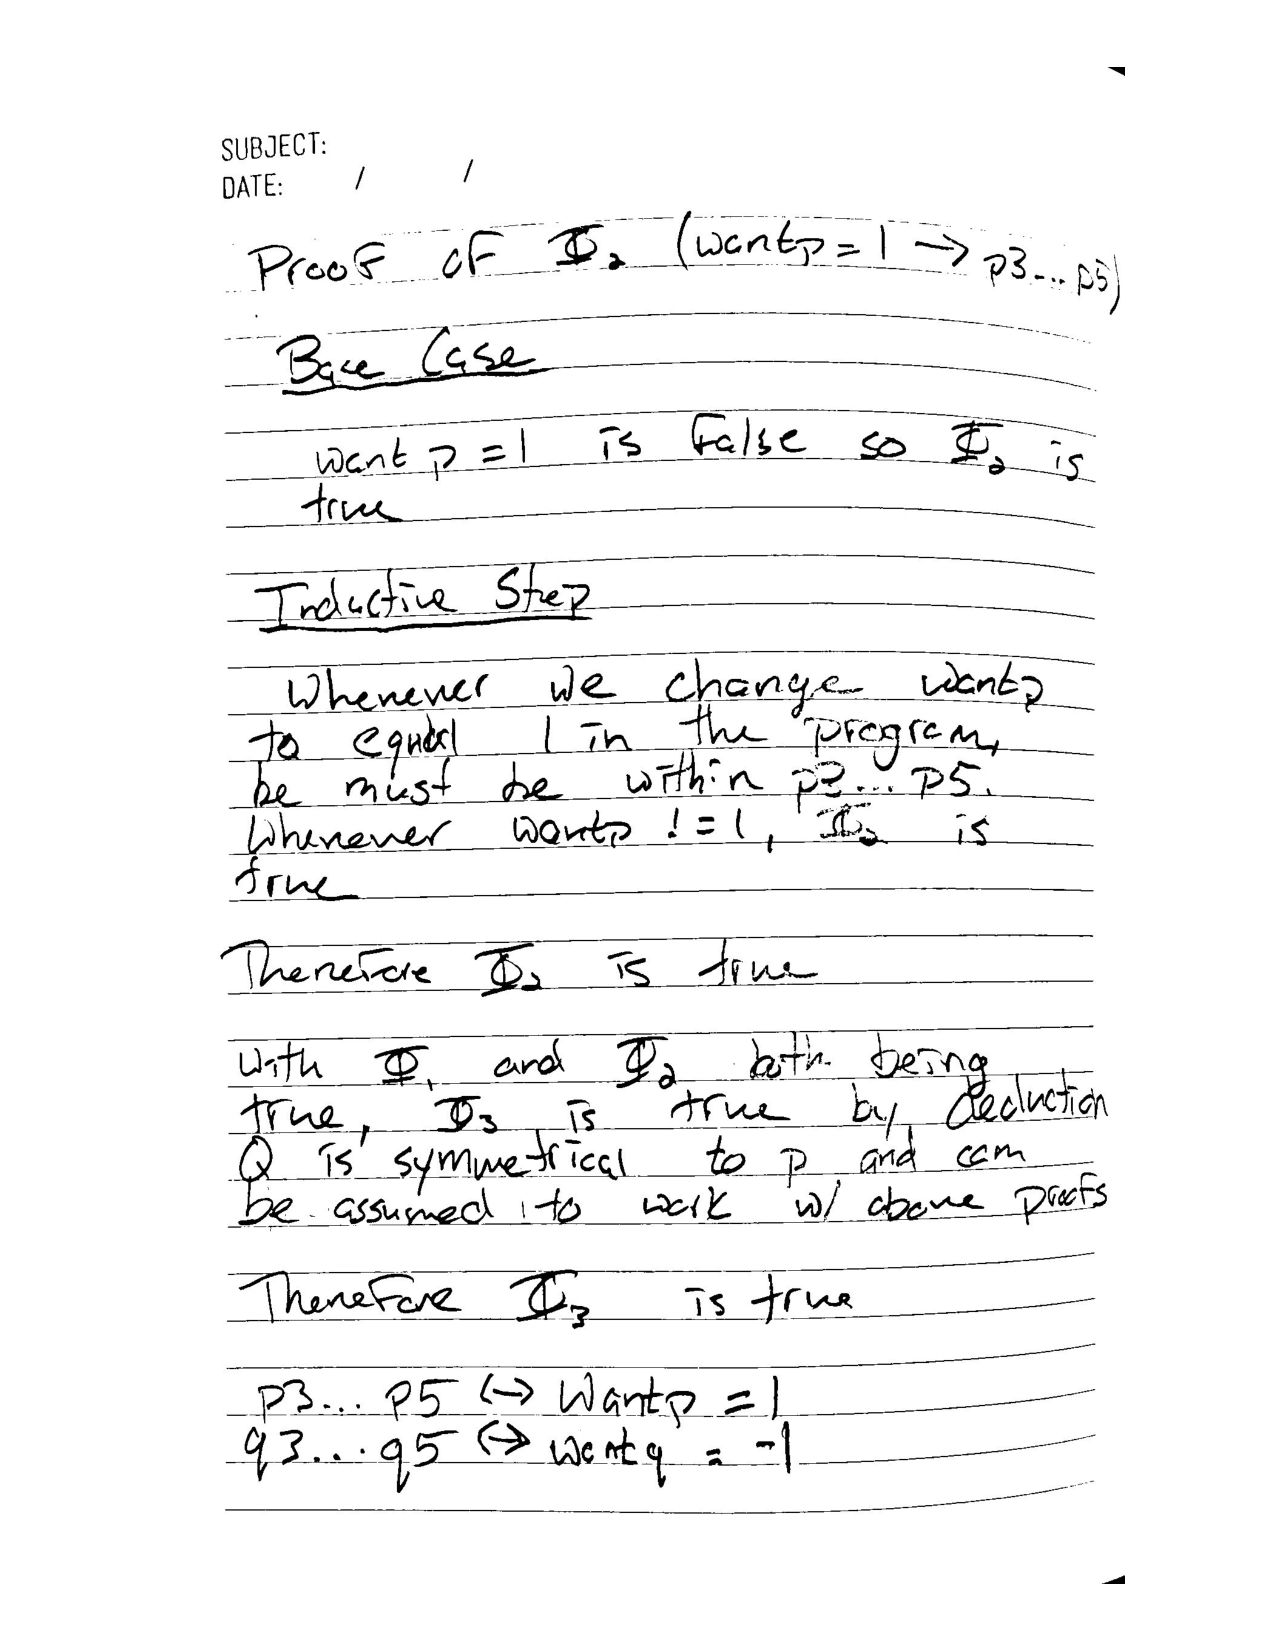
\includegraphics[scale=0.8]{Assignment3/2.pdf}
        \newpage
        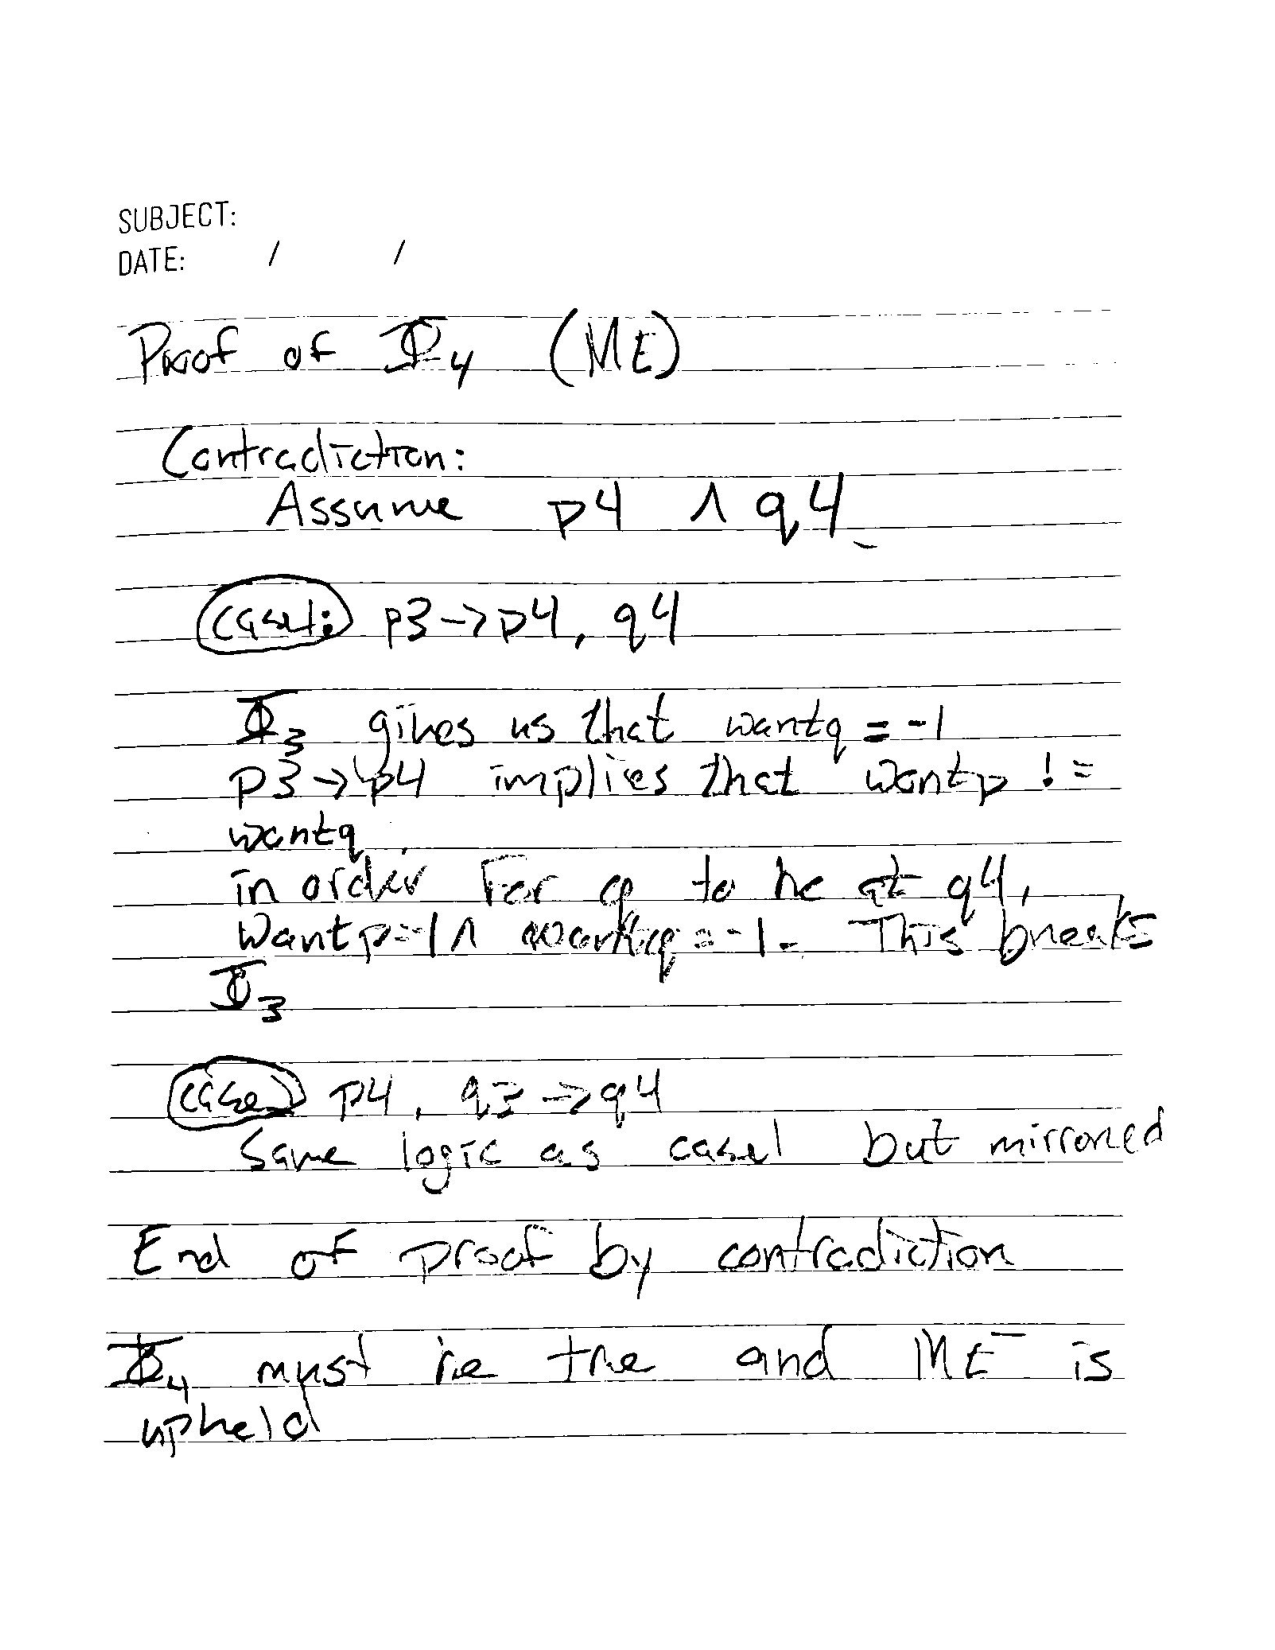
\includegraphics[scale=0.8]{Assignment3/3.pdf}
        \newpage

        
    \section{Part 2 - Report}
        Description of classes and methods
        \begin{enumerate}
            \item Resident Class \\
                Resident is an abstract class and holds all of the shared data members for any of the actors in this simulation. Resident also outlines some common methods described below
                \begin{enumerate}
                    \item \textit{eatFood()} - generates a random amount of food for the Resident to consume between \textit{cfmin} and \textit{cfmax} and subtracts it from the Resident's food store \textit{nf}. If the amount that is generated is greater than the amount of food that the Resident has in their food store, they will not eat that day.
                    \item \textit{getBuyFoodAmount()} - returns a random amount of food for the Resident to buy based on \textit{bfmin} and \textit{bfmax} \\
                    \item \textit{shop()} - requests to but this Resident in the shopping queue. This should only happen if the amount of food that the resident has falls below a certain threshold (\textit{fmin}). 
                    \item \textit{nonWork()} - simulates the Resident 'resting', or doing whatever they wish at home. This method just sleeps for a random amount of time between 1 and \textit{smax} * 1000.
                \end{enumerate}
                Resident also has a Semaphore called \textit{waiting} which can be used by any other Resident. The idea here is that this Semaphore will start at 0. When the Resident is interacting with any other worker, \textit{waiting} can be used to block until the action is completed. For example, when a Farmer is waiting for a Trucker to arrive to pick up the delivery, the Farmer can call \textit{acquire()} on the \textit{waiting} Semaphore and block itself. After the Trucker is finished loading the food on to their truck, they can call \textit{release()} on the Farmer's \textit{waiting} Semaphore to free up the lifecycle of the Farmer.
            \item GroceryStore Class \\
                This class is mainly used to handle all of the synchronization efforts between the GroceryWorkers, Farmers, and Truckers. GroceryStore has methods which are described below
                \begin{enumerate}
                    \item \textit{clockOut()} - a GroceryWorker will clock out when their shift is over with. This method simply prints out what employee is clocking out and decrements the \textit{currentWorkerCount}
                    \item \textit{wantToWork()} - this method is called when GroceryWorkers are attempting to shop up to work for the day. It increments the amount of \textit{currentWorkers} and will block the GroceryWorker if there are not enough workers available in the store. When enough workers have requested to begin working, all of the GroceryWorkers are have their \textit{waiting} Semaphore called \textit{release()}.
                    \item \textit{getInLine()} - adds a Resident to the queue of Residents in line at the store. If the store is full, the Resident is blocked, and waits until they are able to get a spot in the line. The queue of Residents acts as a bounded buffer of fixed size \textit{sc}.
                    \item \textit{serviceCustomer} - this is the main working lifecycle loop for the GroceryWorkers. While the store is open, they are constantly calling this method. This method acts as a consumer of the bounded buffer of Residents waiting to be served. This is the method that gets the amount of food that the resident wishes to buy, and subtracts that amount from the store. Since only one customer is allowed in the store, there is a Semaphore that acts as a mutex that locks the critical section of being served. This method is also responsible for determining whether or not the maximum amount of customers have been served for the day. If we reach that limit, then the GroceryWorkers will go home and the Residents who are waiting in line will block.
                    \item \textit{acceptDeliver()} - is responsible for handling a delivery of food from a Trucker. The amount of food that the trucker has to deliver is removed from the trucker's \textit{currentAmount} and added to the store's capacity.
                \end{enumerate}
            \item Farmer Class \\
            This class is used to coordinate the lifecycle of a farmer. The Farmer class is a Thread, and implements the Runnable interface. Inside of the constructer, the Farmer's lifecycle is started and executes the \textit{run()} method. The Farmer's methods are outlined below.
            \begin{enumerate}
                \item \textit{farm()} - generates a random amount of food and adds it to the farmer's current amount.
                \item \textit{getFoodForTrucker()} - returns the Farmer's \textit{nf}. This is needed so that Trucker can determine if there is enough room on his truck in order to complete the delivery
                \item \textit{awaitTruckerToTakeFood()} - blocks until a Trucker is available to pickup the food that the farmer has generated. There is a bounded buffer that is used to represent the farmers who are waiting to be serviced by a Trucker. In this method, the Farmers put themselves on this queue so that a Trucker can assist them. The Farmer also calls its own \textit{waiting} Semaphore's \textit{acquire()} method so that the Farmer blocks until a truck appears
                \item \textit{run()} - runs the lifecycle of a Farmer. The lifecycle goes as follows: 
                \begin{enumerate}
                    \item \textit{farm()}
                    \item \textit{eatFood()}
                    \item \textit{awaitTruckerToTakeFood()}
                    \item \textit{shop()}
                    \item \textit{nonWork()}
                \end{enumerate}
            
            \end{enumerate}
            
            \item GrocreyWorker Class \\ 
            This class is used to coordinate the lifecycle of a GroceryWorker. The GroceryWorker class is a Thread, and implements the Runnable interface. Inside of the constructor, the GroceryWorker's lifecycle is started and executes the \textit{run()} method. The GroceryWorker's methods are outlined below.
                \begin{enumerate}
                    \item \textit{beginWorking()} - blocks the GroceryWorker untill the GroceryStore has enough employees. As soon as they become unblocked a print message shows that the GroceryWorker has began working
                    \item \textit{serviceCustomers()} - working loop for the GroceryWorker. This method will loop while the store is open, and constantly attempt to service customers by consuming them off of the bounded buffer \textit{queue}. When the GroceryWorker exits this loop, they can clock out of the GroceryStore.
                    \item \textit{run()} - runs the lifecycle of a GroceryWorker. The lifecycle goes as follows:
                    \begin{enumerate}
                        \item \textit{eatFood()}
                        \item \textit{beginWorking()}
                        \item \textit{serviceCustomers()}
                        \item \textit{shop()}
                        \item \textit{nonWork()}
                    \end{enumerate}
                \end{enumerate}
        
            \item Trucker Class \\
            This class is used to coordinate the lifecycle of a Trucker. The Trucker class is a Thread, and implements the Runnable interface. Inside of the constructor, the Trucker's lifecycle is started and executes the \textit{run()} method. The Trucker's methods are outlined below.
            \begin{enumerate}
                \item \textit{pickupFood()} - pops a Farmer off of the bounded buffer \textit{waitingFarmers} and gets the amount of food that the Farmer has. If the trucker does not have enough space on their Truck, they will take as much food as they can that fills the truck, and continue on. After collecting the food, the Farmer's \textit{waiting} Semaphore has \textit{release()} called so that they can continue their lifecycle.
                \item \textit{deliverFood()} - delivers all of the food that the Trucker has to the GroceryStore. Calls the GroceryStore class's \textit{acceptDeliver()} method
                \item \textit{run()} - runs the lifecycle of a Trucker. The lifecycle goes as follows:
                \begin{enumerate}
                    \item \textit{eatFood()}
                    \item \textit{pickupFood()}
                    \item \textit{deliveryFood()}
                    \item \textit{shop()}
                    \item \textit{nonWork()}
                \end{enumerate}
            \end{enumerate}
        \end{enumerate}
        
        
\end{document}
